\section{Applications of EM: Conditional Generation}
\begin{definition}[Generation]
    Given data vectors $\mathbf{x}_1,\mathbf{x}_2,\dots,\mathbf{x}_n\in\R^d$ sampled IID from a known pdf $p$ with parameters $\theta$, solving for $\theta$ allows more IID samples to be generated from $\mathbf{x}$. \textbf{Conditional generation} assumes there exists a set of possible classes $\mathcal{C}=\{1,2,\dots,k\}$ where $p(x,c;\theta)$ is modeled instead. Knowing the priors $\p(c)$, we are able to model the condition distribution $p(x|c;\theta)$. \textbf{Unsupervised conditional generation} further assumes that we are not given access to the $c$, requiring us to model the clustering of our input for generation. The latter case will be the primary focus of this section.
\end{definition}
\subsection{Pure Gaussian Mixture Models}
Gaussian Mixture fitting with the EM algorithm allows $\mathbf{x}_1,\mathbf{x}_2,\dots,\mathbf{x}_n\in\R^d$ to be modeled with a cluster of Gaussian distribution. During inference time, one could sample from one of the Gaussian cluster conditioned on one of the available class for unsupervised conditional generation. This comes with severe limitations as previously established, as Gaussian Mixture models are prone to local optima as a result of poor starting condition while requiring the input dataset to be virtually noise-free. 

\subsection{Conditional Variational Autoencoders}
Variational Autoencoders allows the $p(x,\mathbf{z};\theta)$ to be learned and sampled from, fulfilling the generation task. Still, a glaring limitation remains with the Gaussian limitation of the latent space ($p(\mathbf{z};\theta)$ is $\normal(\mathbf{0},\mathbf{I_s})$). In this section, we aim to survey existing works that generalizes the latent space to a support discrete sampling from a set of classes $\mathcal{C}=\{1,2,\dots,k\}$.

\subsubsection{The M2 Model}
The paper ``Semi-supervised Learning with Deep Generative Models'' \cite{m2} generalizes the regular VAE's latent space with the following assumptions during the sampling process
\begin{itemize}
    \item Sampled data can take $k$ different classes $\mathcal{C}=\{1,2,\dots,k\}$.
    \item The prior is modeled by two latent components $c\in\mathcal{C}$ and $\mathbf{z}\in\R^s$ instead of just $\mathbf{z}$
    \item Given $p(c;\theta)\sim\text{Categorical}(\mathcal{C})$ (assumed to be of equal probability) and $p(\mathbf{z};\theta)\sim\normal(\mathbf{0},\mathbf{I_s})$ (the latter being the exact same as the VAE), we aim to model $p(\mathbf{x},\mathbf{z},c;\theta)$ and the corresponding $q(\mathbf{z},c|\mathbf{x};\phi)$
\end{itemize}
This model, dubbed the M2 model in the paper (since M1 refers to the original VAE), assumes that distinct pdf's $p(\mathbf{x}|\mathbf{z},c;\theta)$ can be modeled conditional on $c$ discretely in addition to a continuous latent $\mathbf{z}$. For the case of image generation, this could be conditioning the generation to a cat via $c$, and the breed of said cat via $\mathbb{z}$. To model the training objective, the authors first consider a supervised setting, one where $c$ is given:
\begin{align*}
    \text{ELBO}(\mathbf{x},c,\theta,\phi)
    &= \E_{z\sim q(\mathbf{z}|\mathbf{x},c;\phi)}\left[\log\left(\frac{p(\mathbf{x},\mathbf{z},c;\theta)}{q(\mathbf{z}|\mathbf{x},c;\phi)}\right)\right] \\
    &= \E_{z\sim q(\mathbf{z}|\mathbf{x},c;\phi)} [\log(p(\mathbf{x}|c,\mathbf{z};\theta))+\log(p(c;\theta))+\log(p(\mathbf{z};\theta))-\log(q(\mathbf{z}|\mathbf{x},c))]\\
    &= -\mathcal{L}(\mathbf{x},c)
\end{align*}
This is the regular reconstruction + KL divergence formulation of the VAE while additionally conditioning the decoder on $c$. The authors then further generalizes the term in the case where $c$ is not given, resulting in the expression
\begin{align*}
    \text{ELBO}(\mathbf{x},\theta,\phi)
    &= \sum_{c\in\mathcal{C}} q(c|\mathbf{x};\phi) (-\mathcal{L}(\mathbf{x},c) + \mathcal{H}(q(c|\mathbf{x};\phi)) )
\end{align*}
When $\mathcal{H}(q(c|\mathbf{x};\phi))$ denotes the conditional entropy of $c$ given $\mathbf{x}$ under the classification of $q,\phi$. This term optimizes when $q(c|\mathbf{x};\phi)$ is uniform, which refers to how an unlabeled sample is as likely to be of any class. In a semi-supervised setting, we are given labeled samples to learn $q(c|\mathbf{x};\phi)$, hence $-\mathcal{L}(\mathbf{x},c)$ is updated most in the it's most likely class. However, in an unsupervised setting, $q(c|\mathbf{x};\phi)$ is learned during the optimization of $\text{ELBO}(\mathbf{x},\theta,\phi)$ where the class with the highest ELBO is the most likely to be predicted. 
\subsubsection{The GMVAE Model}
The paper ``Deep Unsupervised Clustering with Gaussian Mixture Variational Autoencoders'' \cite{gmvae} further generalizes the latent space into a Gaussian Mixture Model as follows:
\begin{itemize}
    \item Sampled data can take $k$ different classes $\mathcal{C}=\{1,2,\dots,k\}$.
    \item The prior is modeled by two latent components $c\in\mathcal{C}$ and $\mathbf{z}\in\R^s$ instead of just $\mathbf{z}$
    \item Given $p(c;\theta)\sim\text{Categorical}(\mathcal{C})$ (assumed to be of equal probability) and $p(\mathbf{z}_1;\theta)\sim\normal(\mathbf{0},\mathbf{I_s})$, we model $\mathbf{z}_2$ as a Gaussian Mixture Model where the class weights are $p(c;\theta)$ with means $\mu_\theta(\mathbf{z}_1)$ and covariances $\text{diag}(\sigma^2_\theta(\mathbf{z}_1))$ conditioned on $\mathbf{z}_1$, that is, $\mathbf{z}_2|\mathbf{z}_1,c$ is a Gaussian Mixture Model.
    \item Likewise, we aim to learn $p(\mathbf{x},\mathbf{z}_1,c,\mathbf{z}_2;\theta)$ and the corresponding $q(\mathbf{z}_1,c,\mathbf{z}_2|\mathbf{x};\phi)$
\end{itemize}
This model, dubbed the Gaussian Mixture VAE (GMVAE), implicitly uses a Gaussian Mixture model as its latent space since only the conditional latent follows a Gaussian Mixture model. Likewise, the author derived the ELBO for this model, which can be expressed like below:
\begin{align*}
    \mathrm{ELBO}(\mathbf{x},\theta,\phi)
    &= \mathbb{E}_{c \sim q(c \mid \mathbf{x}; \phi)}\bigl[\log p(\mathbf{x} \mid c; \theta)\bigr] \\[6pt]
    &\quad
    - \mathbb{E}_{\mathbf{z}_1,\,c \sim q(\mathbf{z}_1 \mid \mathbf{x}; \phi)\,p(c \mid \mathbf{z}_2,\mathbf{z}_1; \theta)}
    \bigl[D_{\mathrm{KL}}\bigl(q(c \mid \mathbf{z}_2,\mathbf{x}; \phi),\,p(c \mid \mathbf{z}_2,\mathbf{z}_1; \theta)\bigr)\bigr] \\[6pt]
    &\quad
    - D_{\mathrm{KL}}\bigl(q(\mathbf{z}_1 \mid \mathbf{x}; \phi),\,p(\mathbf{z}_1)\bigr) \\[6pt]
    &\quad
    - \mathbb{E}_{c,\,\mathbf{z}_1 \sim q(c \mid \mathbf{x}; \phi)\,q(\mathbf{z}_1 \mid \mathbf{x}; \phi)}
    \bigl[D_{\mathrm{KL}}\bigl(p(c \mid \mathbf{z}_2,\mathbf{z}_1; \theta),\,p(c \mid \mathbf{z}_2; \theta)\bigr)\bigr]
\end{align*}
We are left with one reconstruction term $\mathbb{E}_{c \sim q(c \mid \mathbf{x}; \phi)}\bigl[\log p(\mathbf{x} \mid c; \theta)\bigr]$ and three KL divergence terms which computes the KL divergence of $\mathbf{z}_1,c$ under different parametrization (note that the author's derivation does not end up with a divergence term for $\mathbf{z}_2$, which would otherwise be intractable as $\mu_\theta(\mathbf{z}_1)$ and $\sigma^2_\theta(\mathbf{z}_1)$ are both unknown). The authors remarked that, like the reconstruction term, the expectation of KL divergence terms could not be directly computed and are instead optimized stochastically with monte-carlo samples.

The authors additionally pointed out the dominance of $c$-termed KL divergence, leading to an undesirable optima where these terms dominate the reconstruction. A solution proposed in this paper and the one prior is to set a cut-off, where the terms are incorporated if and only if they are above that threshold.

\subsection{Comparison}

We first verify that VAEs are able to generate data akin to those being sampled from the dataset. \texttt{code/categorical-generation/vae.ipynb} details the Implementation of a standard VAE, in which the underlying neural network architecture will be used with other implementations. Figure \ref{fig:vae} depicts such generations from the MNIST dataset.

\begin{figure}[h]
    \centering
    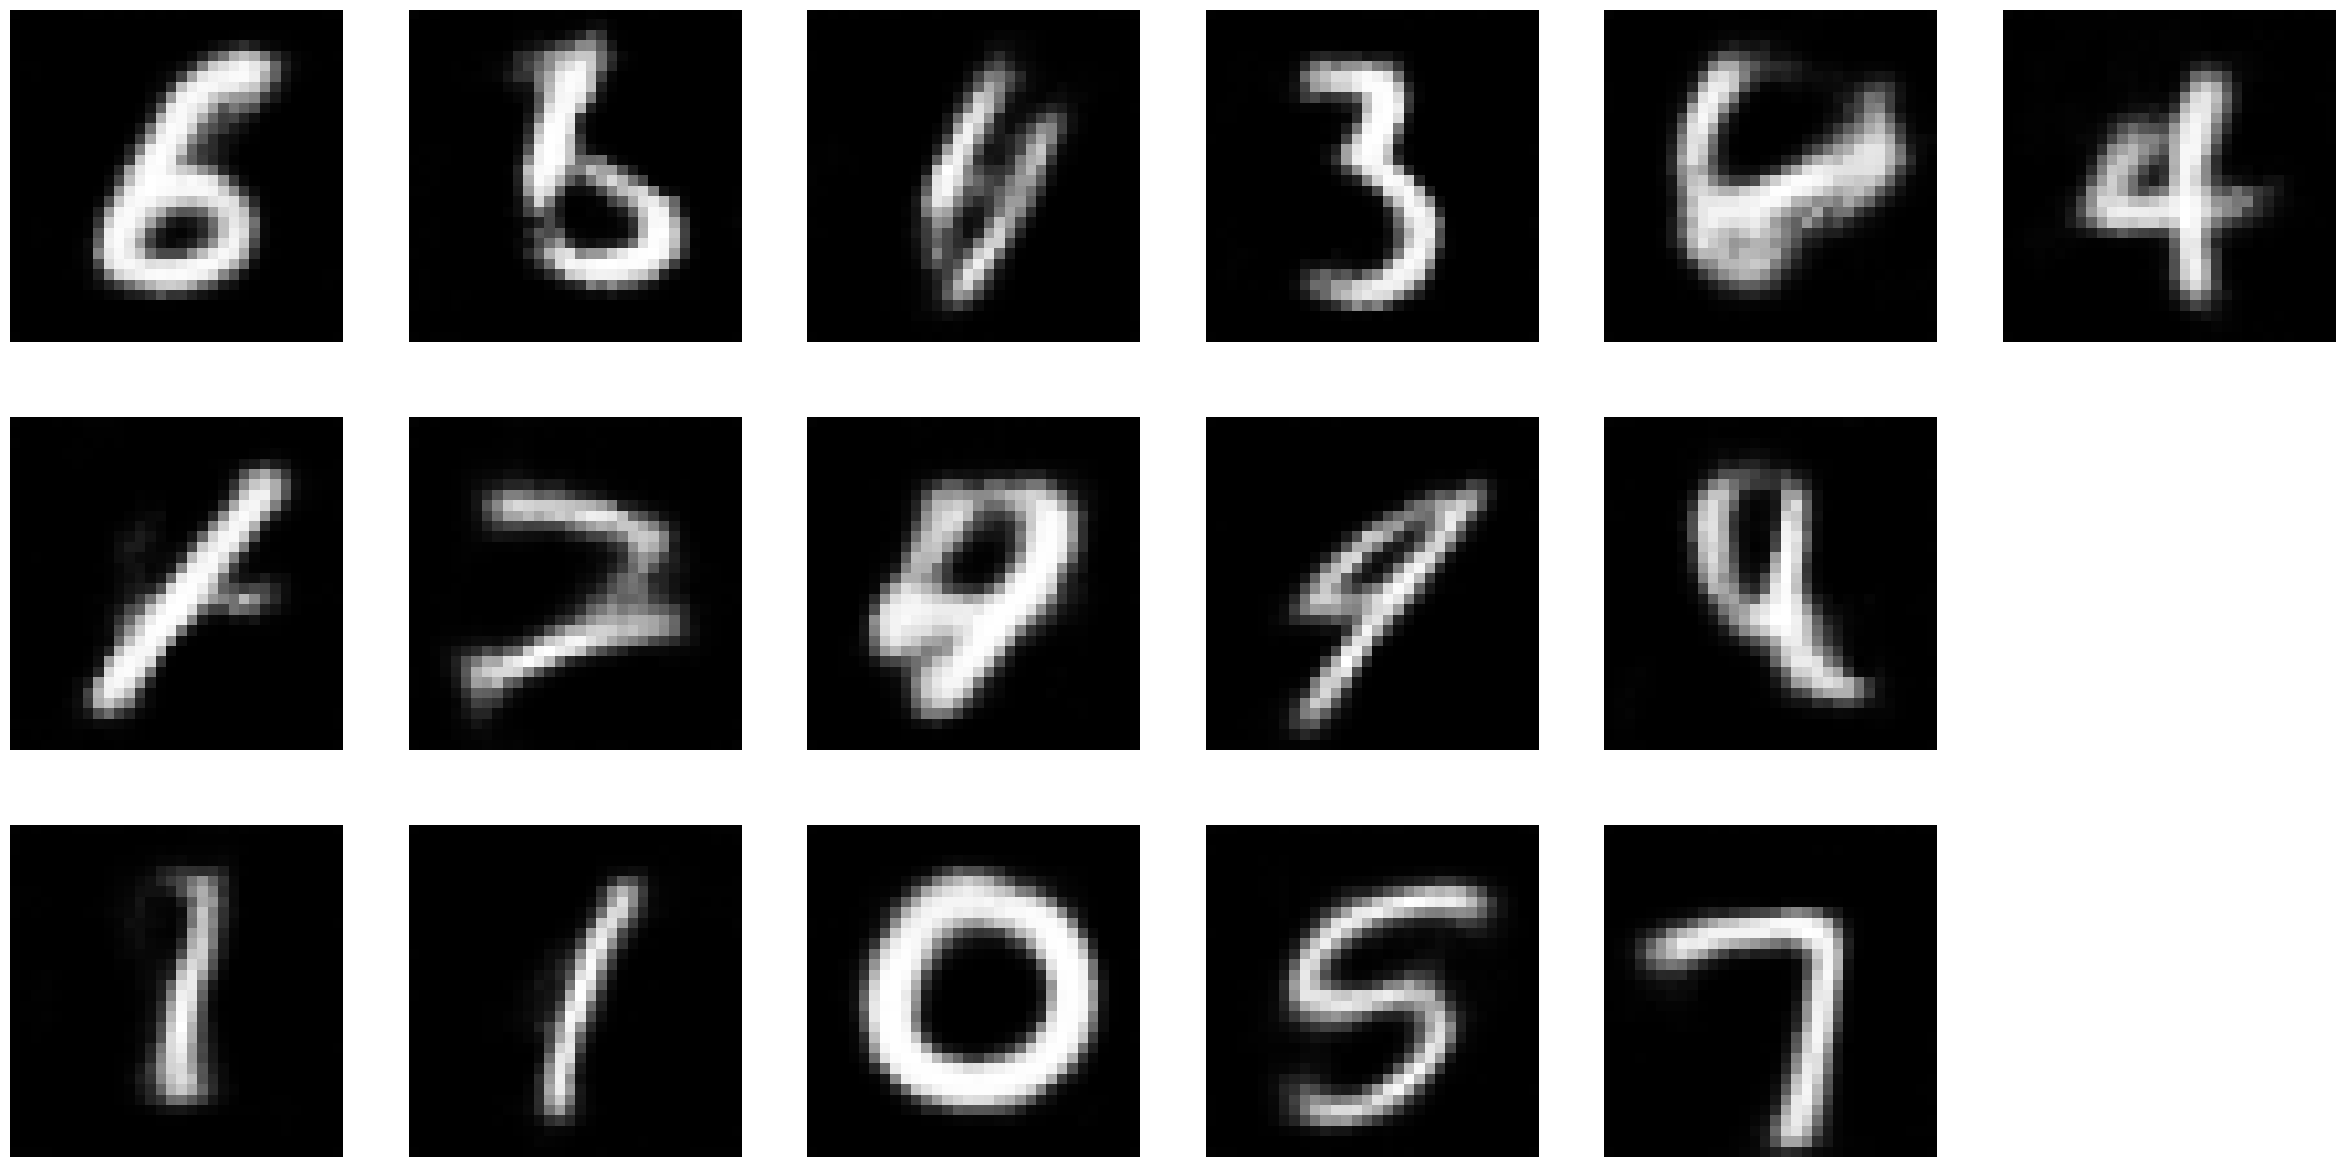
\includegraphics[width=0.6\linewidth]{figures/vae-gt.png}
    \caption{VAE results}
    \label{fig:vae}
\end{figure}

Figure \ref{fig:m2model} shows the categorical generation capabilities of our M2 model implementation. We notice that, due to the dominance of the $c$ KL divergence term, the classes don't separate well and overfit to select ``templates'' which are not representative of the digits. However, it is important to note that the M2 model is designed to be trained in a semi-supervised setting where small labeled samples guide the unlabeled ones. Having trained the model unsupervised, the less than desirable accuracy is a result of this poor clustering. Still misclassifications share a general trend with the digit's appearances (i.e. 4 being misclassified as 9).

\begin{figure}[h]
    \centering
    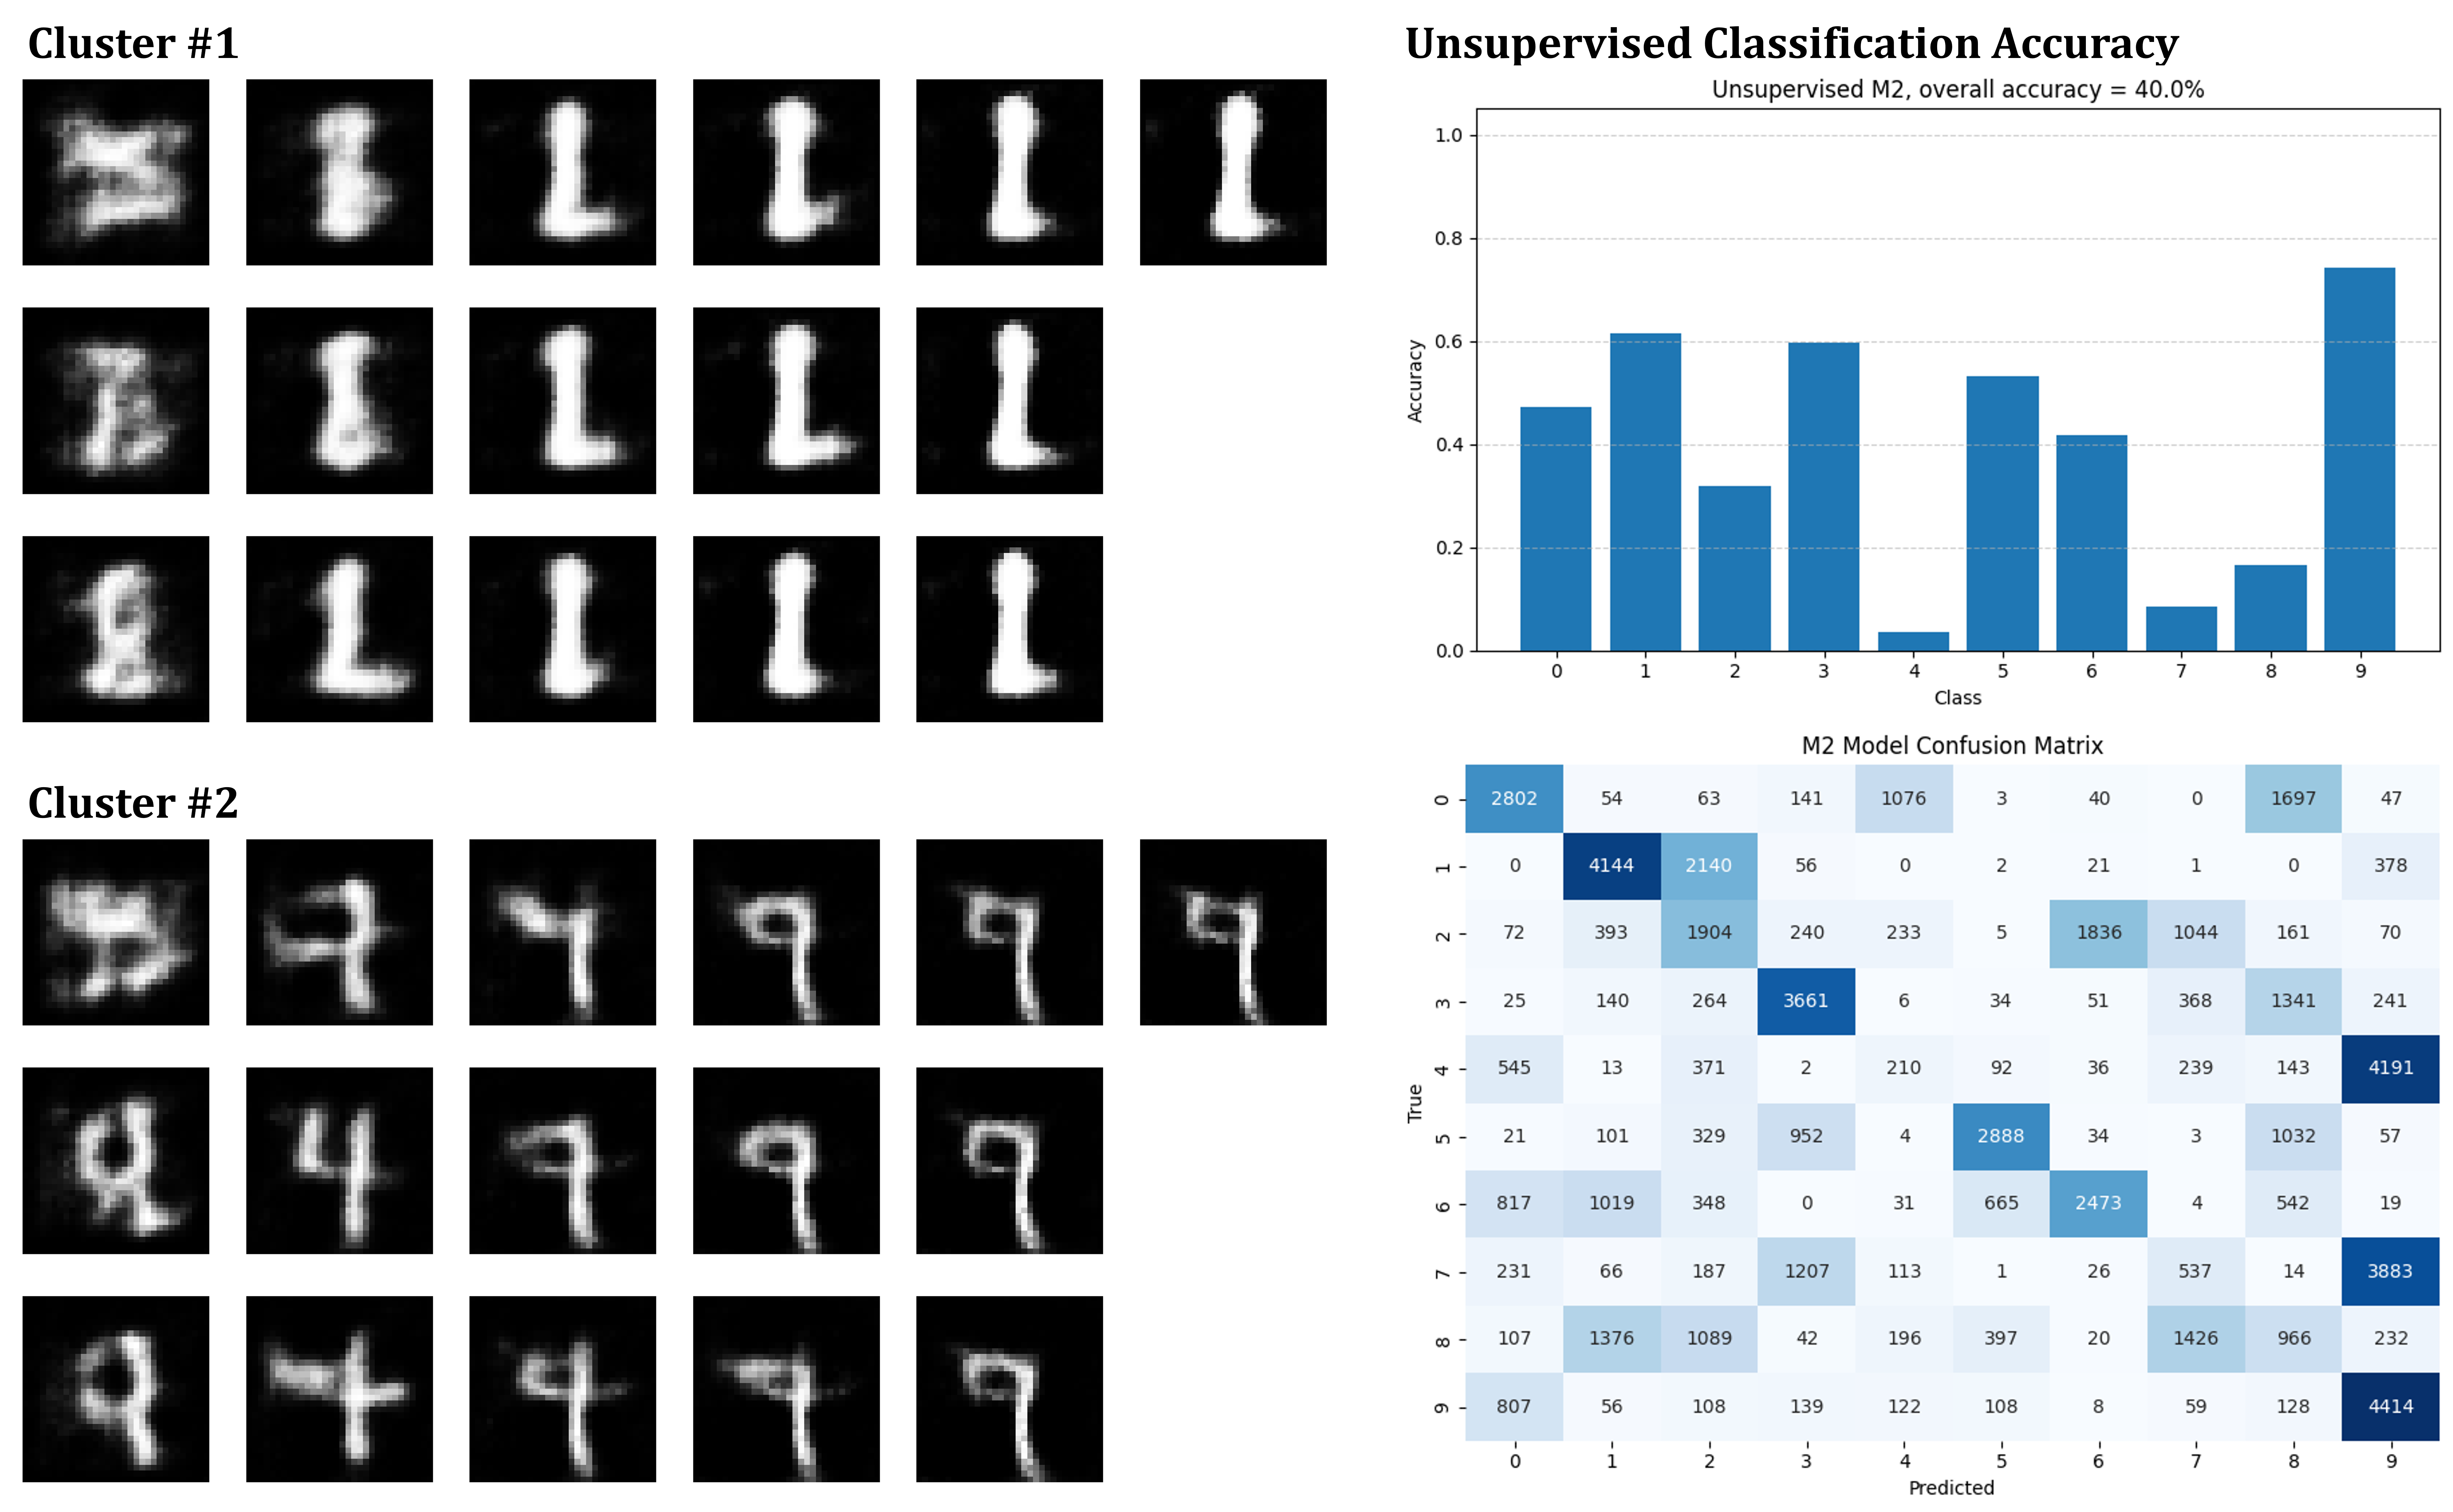
\includegraphics[width=0.9\linewidth]{figures/m2model.png}
    \caption{M2 VAE results}
    \label{fig:m2model}
\end{figure}

Figure \ref{fig:gmvae} shows our attempt at reproducing the results from \cite{gmvae}. While we are able to train a successful VAE, the model does not show impressive clustering capabilities like the original paper. Instead, we notice a subtle pattern between images generated when conditioned with the same $c$. This is because $q(\mathbf{z}_2|\mathbf{z}_1,c)$ is only optimized indirectly, and more specific training conditions are needed for an exact reproduction. Still, we are able to identify that images from the same $c$ share a common ``style'' (i.e. blurry lines on one of the clusters, thicker strokes on the other).

\begin{figure}[h]
    \centering
    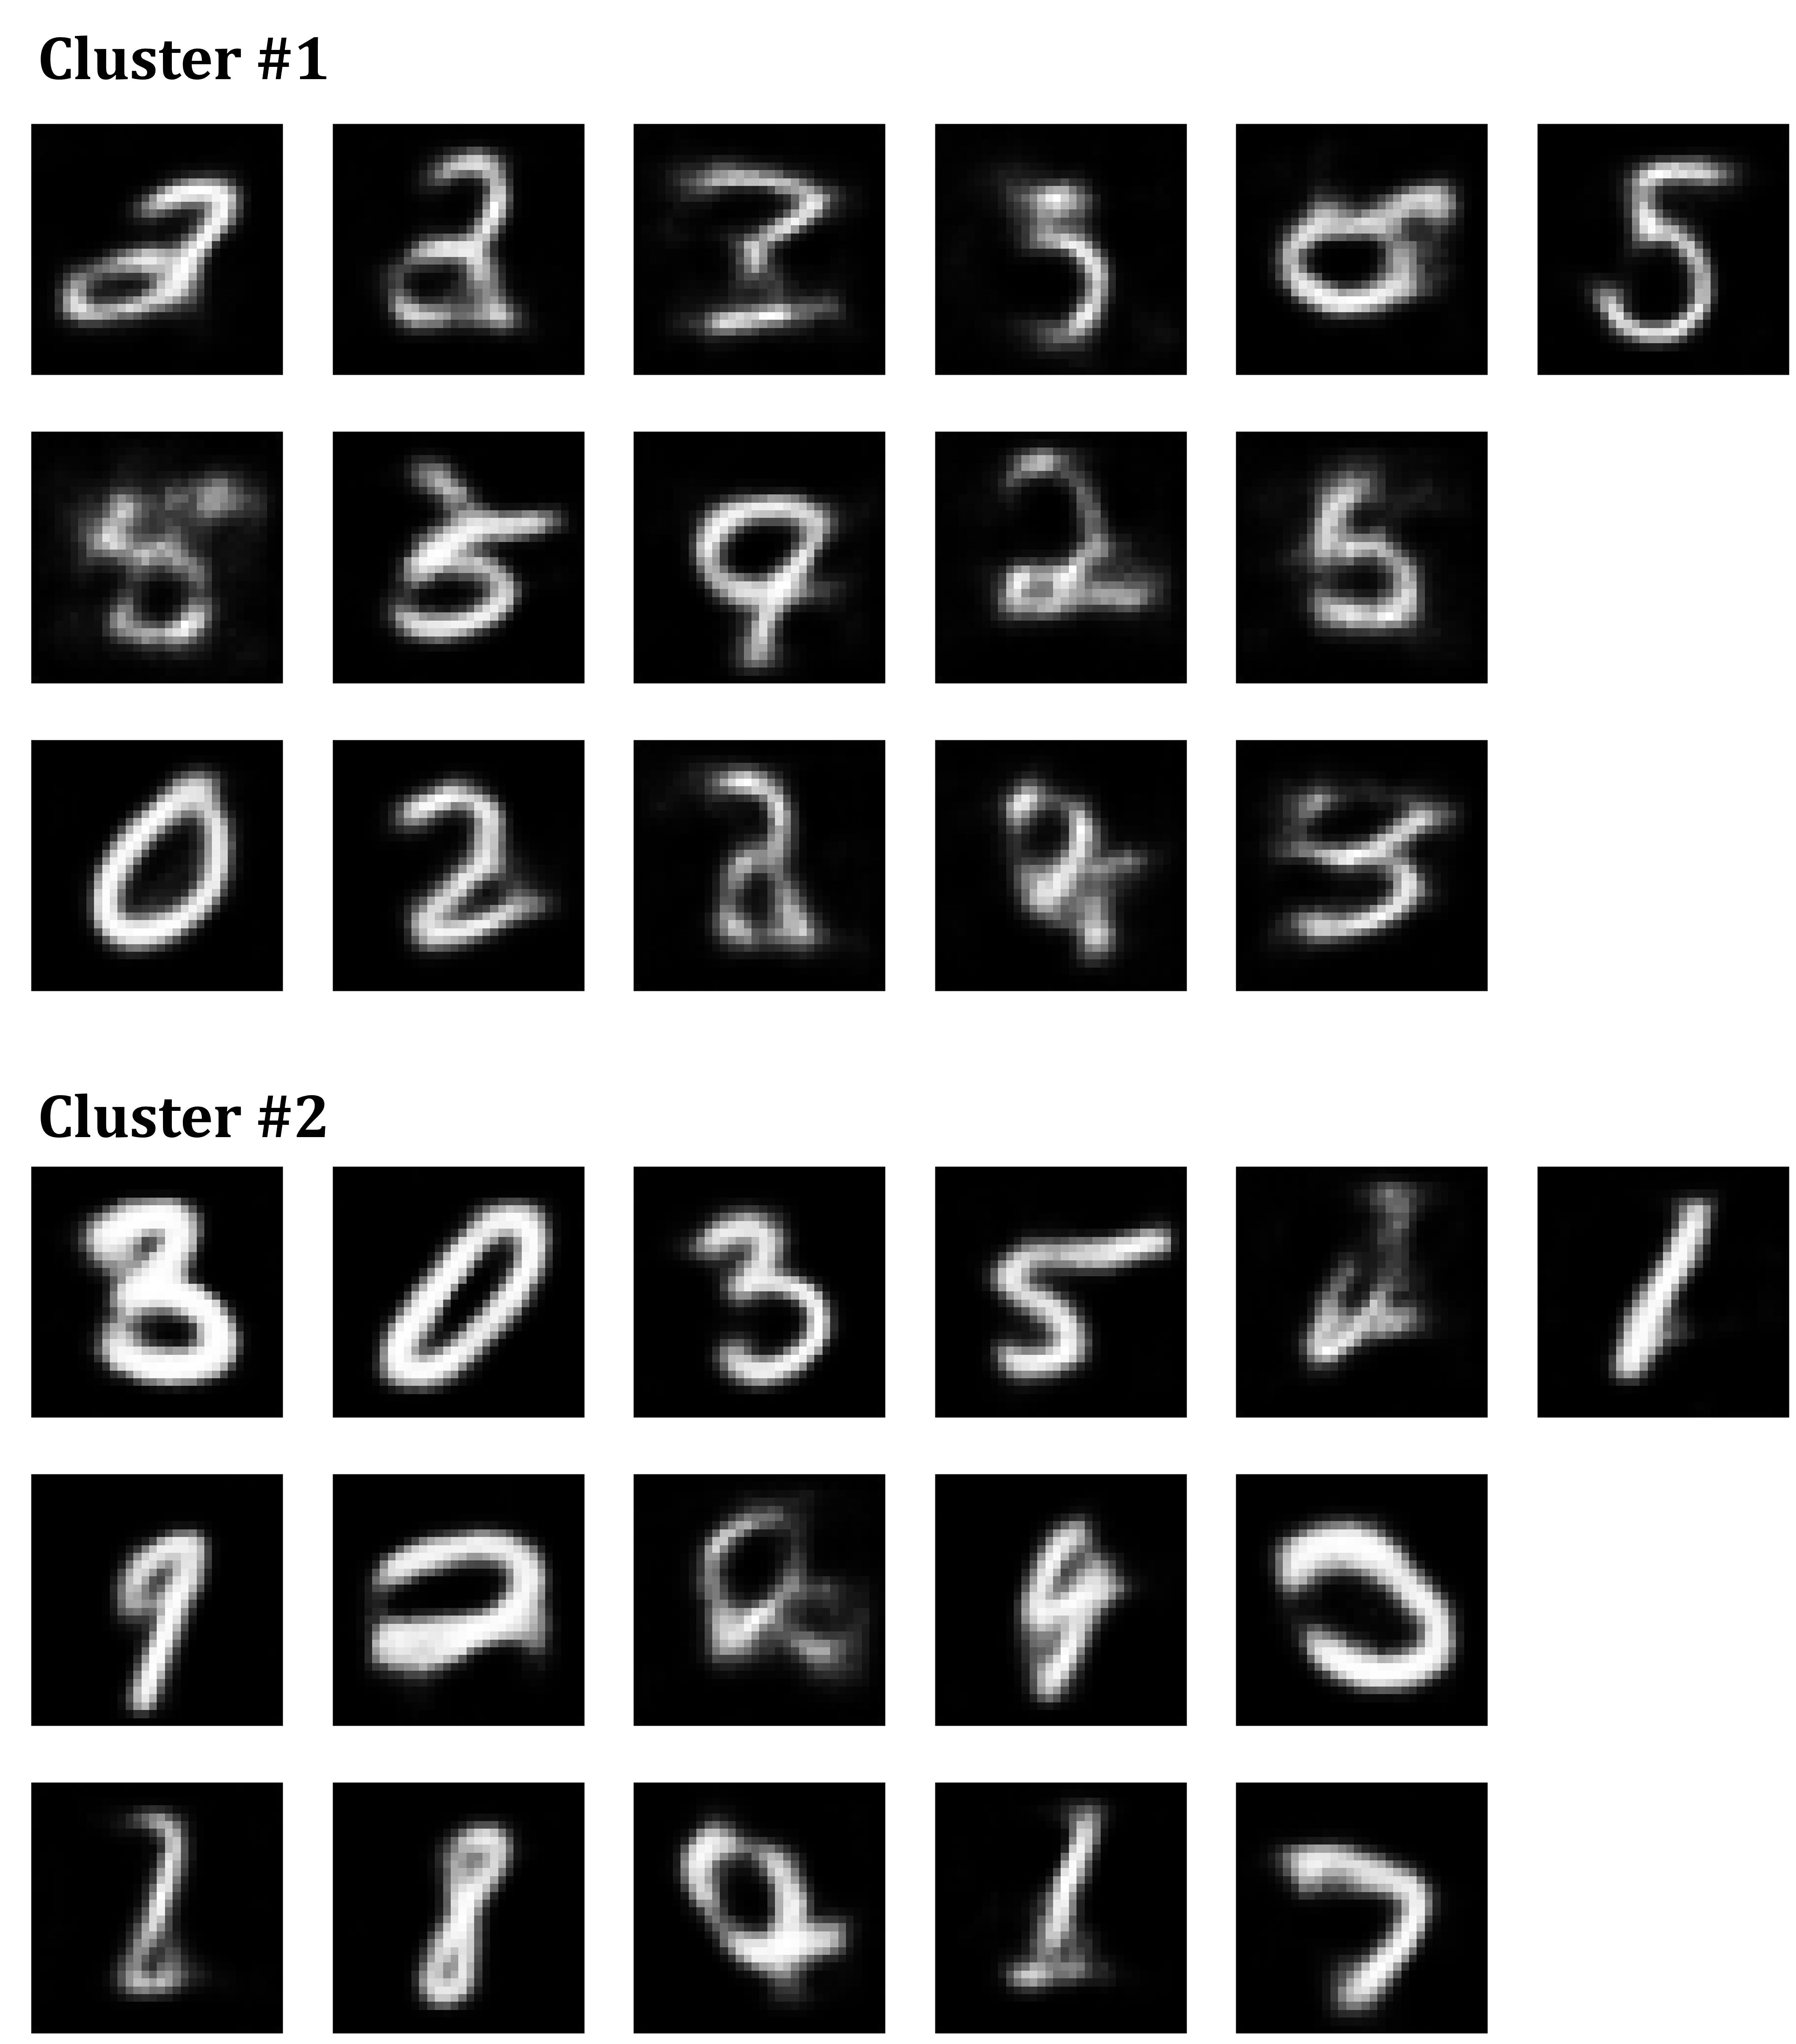
\includegraphics[width=0.9\linewidth]{figures/gmvae.png}
    \caption{GMVAE results}
    \label{fig:gmvae}
\end{figure}